\documentclass[12pt,fleqn]{article}\usepackage{../../common}
\begin{document}



\begin{minted}[fontsize=\footnotesize]{python}
import pandas as pd, zipfile
import numpy as np
import cv2

def draw_flow(img, flow, step=16):
    h, w = img.shape[:2]
    y, x = np.mgrid[step/2:h:step, step/2:w:step].reshape(2,-1).astype(int)
    fx, fy = flow[y,x].T
    lines = np.vstack([x, y, x+fx, y+fy]).T.reshape(-1, 2, 2)
    lines = np.int32(lines + 0.5)
    vis = cv2.cvtColor(img, cv2.COLOR_GRAY2BGR)
    cv2.polylines(vis, lines, 0, (0, 255, 0))
    for (x1, y1), (x2, y2) in lines:
        cv2.circle(vis, (x1, y1), 1, (0, 255, 0), -1)
    return vis

prevgray = cv2.imread('106.jpg', cv2.IMREAD_GRAYSCALE)
gray = cv2.imread('107.jpg', cv2.IMREAD_GRAYSCALE)
flow = cv2.calcOpticalFlowFarneback(prevgray, gray, None, 0.5, 3, 15, 3, 5, 1.2, 0)
cv2.imwrite('vision_30vstab_01.png', draw_flow(gray, flow))
\end{minted}

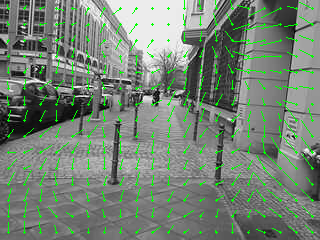
\includegraphics[width=20em]{vision_30vstab_01.png}

\begin{minted}[fontsize=\footnotesize]{python}
x1 = [[25.8064516129,25.0],
      [23.8709677419,45.625],
      [20.0,69.375],
      [28.3870967742,92.5],
      [38.7096774194,116.875],
      [64.5161290323,115.0],
      [64.5161290323,89.375],
      [65.1612903226,66.875],
      [57.4193548387,45.0],
      [45.8064516129,23.75]]
x2 = [[93.5483870968,66.25],
      [114.838709677,110.0],
      [138.709677419,153.125],
      [182.580645161,179.375],
      [241.935483871,204.375],
      [276.774193548,163.75],
      [254.193548387,123.125],
      [212.903225806,73.125],
      [158.064516129,54.375],
      [120.64516129,40.625]]

x1 = np.array(x1)
x2 = np.array(x2)
plt.plot(x1[:,0], x1[:,1], 'r.')
plt.plot(x2[:,0], x2[:,1], 'b.')
plt.xlim(0,320)
plt.ylim(0,240)
plt.savefig('vision_30vstab_02.png')
\end{minted}

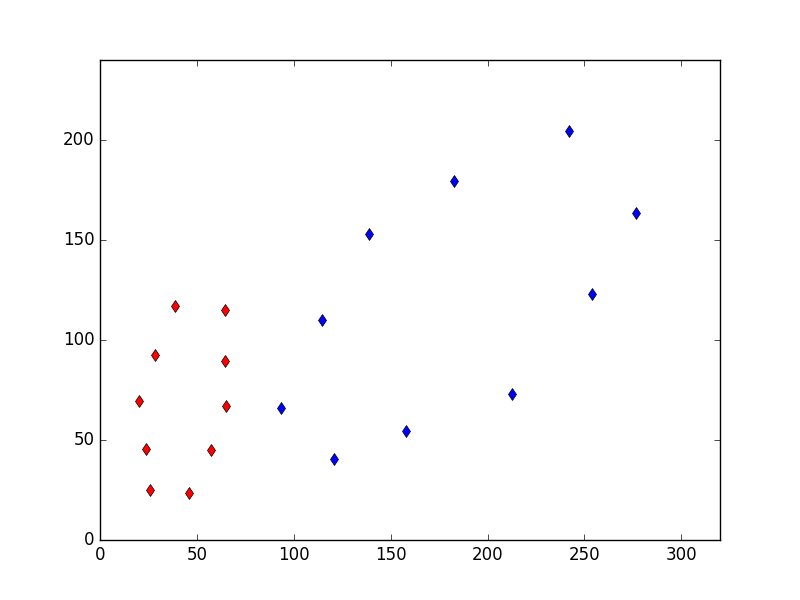
\includegraphics[height=6cm]{vision_30vstab_02.png}

\begin{minted}[fontsize=\footnotesize]{python}
import numpy.linalg as lin

def H_from_points(fp,tp):
    if fp.shape != tp.shape:
        raise RuntimeError('number of points do not match')
        
    m = np.mean(fp[:2], axis=1)
    maxstd = np.max(np.std(fp[:2], axis=1)) + 1e-9
    C1 = np.diag([1/maxstd, 1/maxstd, 1]) 
    C1[0][2] = -m[0]/maxstd
    C1[1][2] = -m[1]/maxstd
    fp = np.dot(C1,fp)
    
    m = np.mean(tp[:2], axis=1)
    maxstd = np.max(np.std(tp[:2], axis=1)) + 1e-9
    C2 = np.diag([1/maxstd, 1/maxstd, 1])
    C2[0][2] = -m[0]/maxstd
    C2[1][2] = -m[1]/maxstd
    tp = np.dot(C2,tp)
    
    nbr_correspondences = fp.shape[1]
    A = np.zeros((2*nbr_correspondences,9))
    for i in range(nbr_correspondences):        
        A[2*i] = [-fp[0][i],-fp[1][i],-1,0,0,0,
                    tp[0][i]*fp[0][i],tp[0][i]*fp[1][i],tp[0][i]]
        A[2*i+1] = [0,0,0,-fp[0][i],-fp[1][i],-1,
                    tp[1][i]*fp[0][i],tp[1][i]*fp[1][i],tp[1][i]]
    
    U,S,V = lin.svd(A)
    H = V[8].reshape((3,3))    
    
    H = np.dot(lin.inv(C2),np.dot(H,C1))
    
    # normalize and return
    return H / H[2,2]

x1h = np.ones((len(x1),3))
x1h[:,:2] = x1
x2h = np.ones((len(x1),3))
x2h[:,:2] = x2
A = H_from_points(x1h.T,x2h.T)
res = np.dot(A, x1h.T).T
res = res.T / res[:,2]

plt.plot(x2[:,0], x2[:,1], 'b.')
plt.plot(res.T[:,0], res.T[:,1], 'rx')
plt.xlim(0,320)
plt.ylim(0,240)
plt.savefig('vision_30vstab_03.png')
\end{minted}




























Kaynaklar

[1] Bayramli, Veri 1, \url{https://www.dropbox.com/s/dlcd1ooxyvvp4cv/bwalk1.mp4?dl=1}

[2] Bayramli, Veri 2, \url{https://www.dropbox.com/s/gr4ny0w7lzsdw4s/bwalk1-stab.avi?dl=1}

[3] Solem, {\em Computer Vision with Python}

[4] Nghia Ho, {\em Simple Video Stabilization using OpenCV},
    \url{http://nghiaho.com/?p=2093}

\end{document}
